\documentclass[border=4pt]{standalone}
\usepackage{amsmath}
\usepackage{tikz}
\usetikzlibrary{arrows.meta, positioning, calc, shapes.geometric, backgrounds, fit}
\usepackage{pgfplots}
\pgfplotsset{compat=1.18}
\usepgfplotslibrary{fillbetween}
\definecolor{deepblue}{RGB}{10, 40, 90}
\definecolor{spaceblue}{RGB}{30, 80, 160}
\definecolor{lightgray}{RGB}{245, 245, 248}
\definecolor{accentgold}{RGB}{180, 140, 40}
\definecolor{earthgreen}{RGB}{40, 120, 80}
\definecolor{warnred}{RGB}{170, 40, 40}
\begin{document}
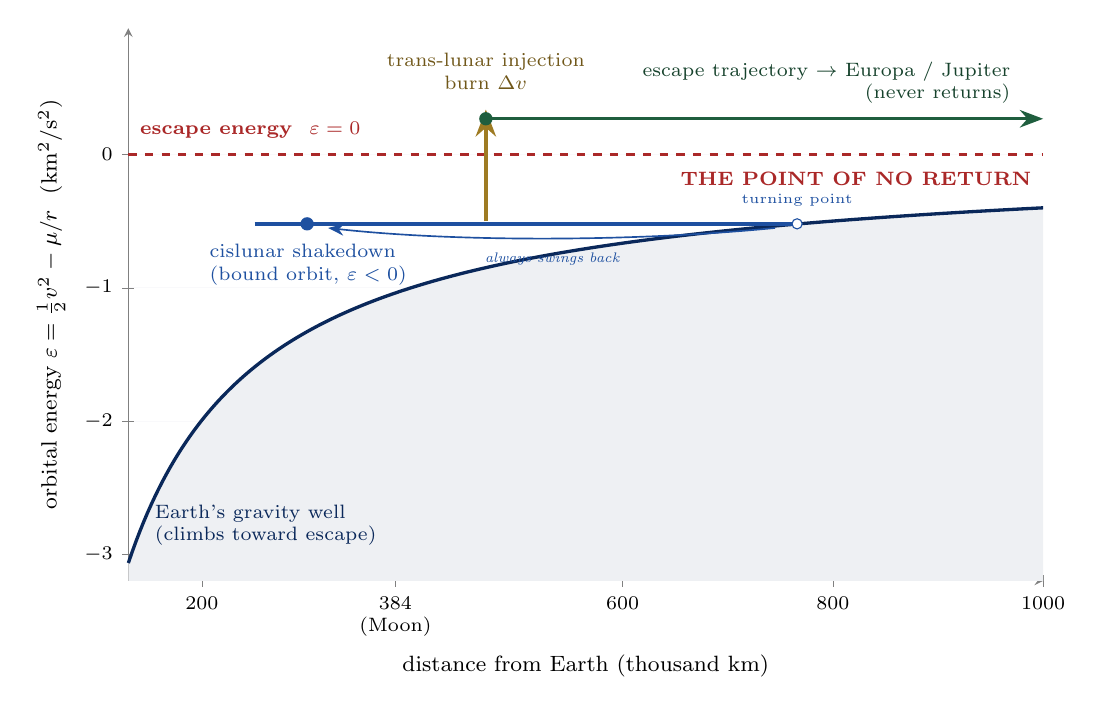
\begin{tikzpicture}
\begin{axis}[
  width=13.2cm, height=8.6cm,
  xlabel={distance from Earth (thousand km)},
  ylabel={orbital energy $\varepsilon = \tfrac{1}{2}v^2 - \mu/r$ \ (km$^2$/s$^2$)},
  xmin=130, xmax=1000, ymin=-3.2, ymax=0.95,
  axis lines=left, axis line style={gray},
  tick label style={font=\scriptsize}, label style={font=\footnotesize},
  ytick={-3,-2,-1,0}, ymajorgrids, grid style={lightgray!60!white},
  xtick={200,384,600,800,1000},
  xticklabels={200,{384\\(Moon)},600,800,1000},
  xticklabel style={align=center},
  clip=false,
]
% --- the gravity well: potential -mu/r, mu = 398600 km^3/s^2, r in 1000 km -> -398.6/x
\addplot[name path=well, deepblue, very thick, domain=130:1000, samples=240] {-398.6/x};
\path[name path=floor] (axis cs:130,-3.2) -- (axis cs:1000,-3.2);
\addplot[deepblue!7] fill between[of=well and floor];
\node[font=\scriptsize, color=deepblue, anchor=west, align=left] at (axis cs:146,-2.78)
  {Earth's gravity well\\(climbs toward escape)};

% --- escape energy: epsilon = 0, the point of no return
\addplot[warnred, very thick, dashed, domain=130:1000] {0};
\node[font=\scriptsize\bfseries, color=warnred, anchor=south west] at (axis cs:132,0.05)
  {escape energy \ $\varepsilon = 0$};
\node[font=\scriptsize\bfseries, color=warnred, anchor=north east, align=right] at (axis cs:998,-0.06)
  {THE POINT OF NO RETURN};

% --- cislunar shakedown: bound level (eps < 0); meets the well at its turning point (x = 766)
\draw[spaceblue, very thick] (axis cs:250,-0.519) -- (axis cs:766,-0.519);
\node[circle, fill=spaceblue, inner sep=1.7pt] at (axis cs:300,-0.519) {};
\node[font=\scriptsize, color=spaceblue, anchor=north west, align=left] at (axis cs:198,-0.6)
  {cislunar shakedown\\(bound orbit, $\varepsilon<0$)};
% turning point + falls-back arrow
\node[circle, draw=spaceblue, fill=white, inner sep=1.3pt] at (axis cs:766,-0.519) {};
\node[font=\tiny, color=spaceblue, anchor=south] at (axis cs:766,-0.46) {turning point};
\draw[-{Stealth}, spaceblue, semithick] (axis cs:745,-0.55) .. controls (axis cs:610,-0.655) and (axis cs:440,-0.655) .. (axis cs:320,-0.55);
\node[font=\tiny\itshape, color=spaceblue, anchor=north] at (axis cs:533,-0.66) {always swings back};

% --- trans-lunar injection: lift the energy level across epsilon = 0
\draw[-{Stealth}, accentgold!88!black, line width=1.5pt] (axis cs:470,-0.5) -- (axis cs:470,0.34);
\node[font=\scriptsize, color=accentgold!62!black, anchor=south, align=center] at (axis cs:470,0.42)
  {trans-lunar injection\\burn $\Delta v$};

% --- post-injection: unbound level (eps > 0), escapes to the right forever
\draw[earthgreen!78!black, very thick] (axis cs:470,0.27) -- (axis cs:980,0.27);
\draw[-{Stealth}, earthgreen!78!black, very thick] (axis cs:980,0.27) -- (axis cs:1000,0.27);
\node[circle, fill=earthgreen!78!black, inner sep=1.7pt] at (axis cs:470,0.27) {};
\node[font=\scriptsize, color=earthgreen!55!black, anchor=south east, align=right] at (axis cs:978,0.31)
  {escape trajectory $\to$ Europa / Jupiter\\(never returns)};
\end{axis}
\end{tikzpicture}
\end{document}
